\documentclass[10pt]{beamer}

\usetheme[progressbar=frametitle]{metropolis}
\usepackage{appendixnumberbeamer}

\usepackage{booktabs}
\usepackage[scale=2]{ccicons}

\usepackage{pgfplots}
\usepgfplotslibrary{dateplot}
\usepackage{caption}
\captionsetup[figure]{labelformat=empty}

\usepackage{xspace}
\newcommand{\themename}{\textbf{\textsc{metropolis}}\xspace}

\title{STDP-based spiking deep convolutional neural networks for object recognition}
\subtitle{Neural Networks}
\date{}
\author{Edoardo Ghini\\Gianluca Cerilli}
\institute{Sapienza Università di Roma}
%\titlegraphic{\hfill
\includegraphics[height=1.cm]{images/SapienzaLogo.pdf}}

\begin{document}

\maketitle

\begin{frame}{Table of contents}
  \setbeamertemplate{section in toc}[sections numbered]
  \tableofcontents[hideallsubsections]
\end{frame}

\section{Introduction}

\begin{frame}[fragile]{Introduction}

Spiking Neural Networks communicate through \textit{spikes}, that are discrete events that occur at certain points in time.\\
\bigskip
When a neuron reaches a certain potential value, it spikes, so it resets its value.\\
\bigskip
This modelling allows us to handle spatio-temporal data,
that are real-world sensory data.

\end{frame}

\section{Network architecture}

\begin{frame}{Architecture}

STDP-based spiking deep neural network (SDNN) with a spike-time neural coding:

\begin{figure}[h]
	\centering
	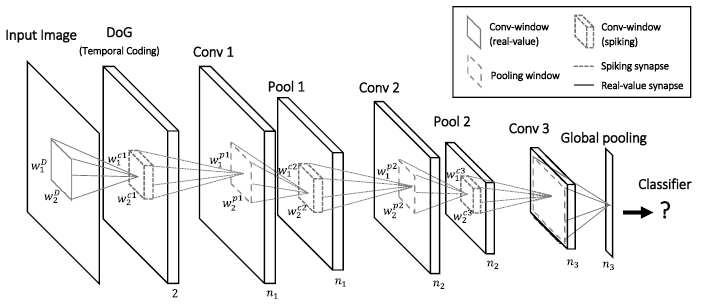
\includegraphics[width=\textwidth]{images/architecture}
\end{figure}

\end{frame}

\begin{frame}{Temporal coding}

Input signal is encoded into temporal-discrete spike events.

\begin{itemize}
	\item A Difference of Gaussians (DoG) filter detects the contrasts
	in the input image and emit a spike, accordingly.
	
	\item The higher the contrast in a cell, the more strongly this one is activated in order to fire.
	
	\item The firing time $ \tau = 1/r $ of a cell is inversely proportional to its activation value \textit{r}.
\end{itemize}

\end{frame}

\begin{frame}{Temporal coding}

\begin{columns}
	\column{.5\textwidth}
	\begin{figure}[!h]
		\centering
		\caption{DoG temporal coding (human face)}
		\begin{minipage}[b]{\textwidth}
			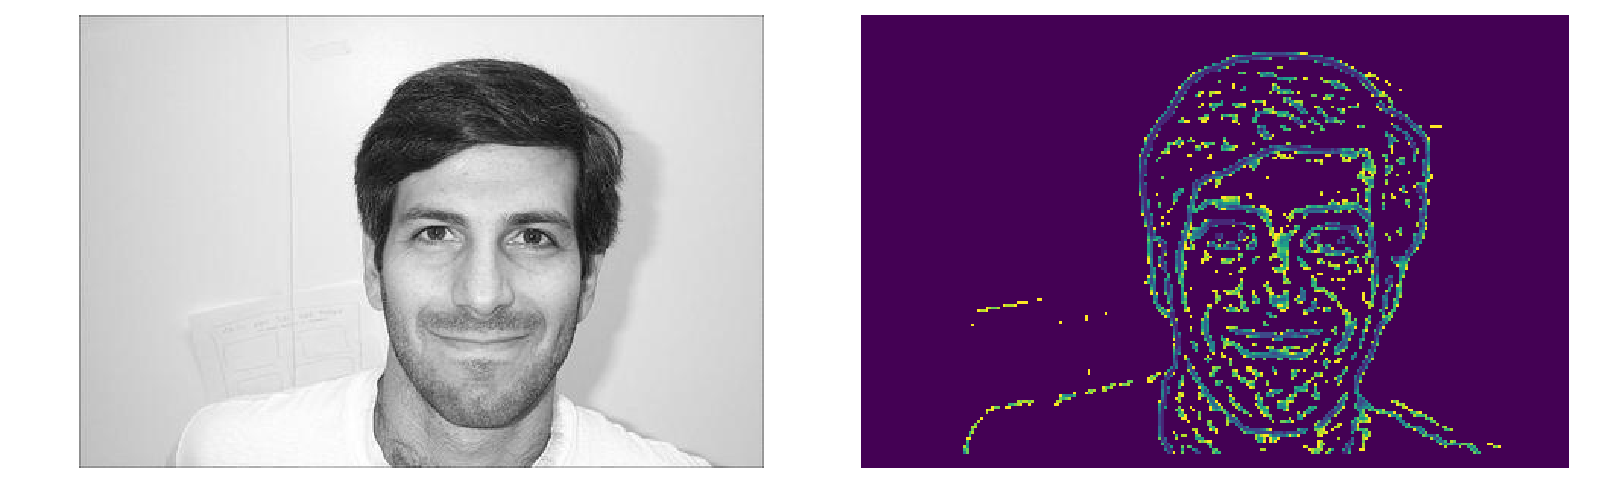
\includegraphics[width=\textwidth]{images/face_temp}
		\end{minipage}
		\\
		\begin{minipage}[b]{\textwidth}
			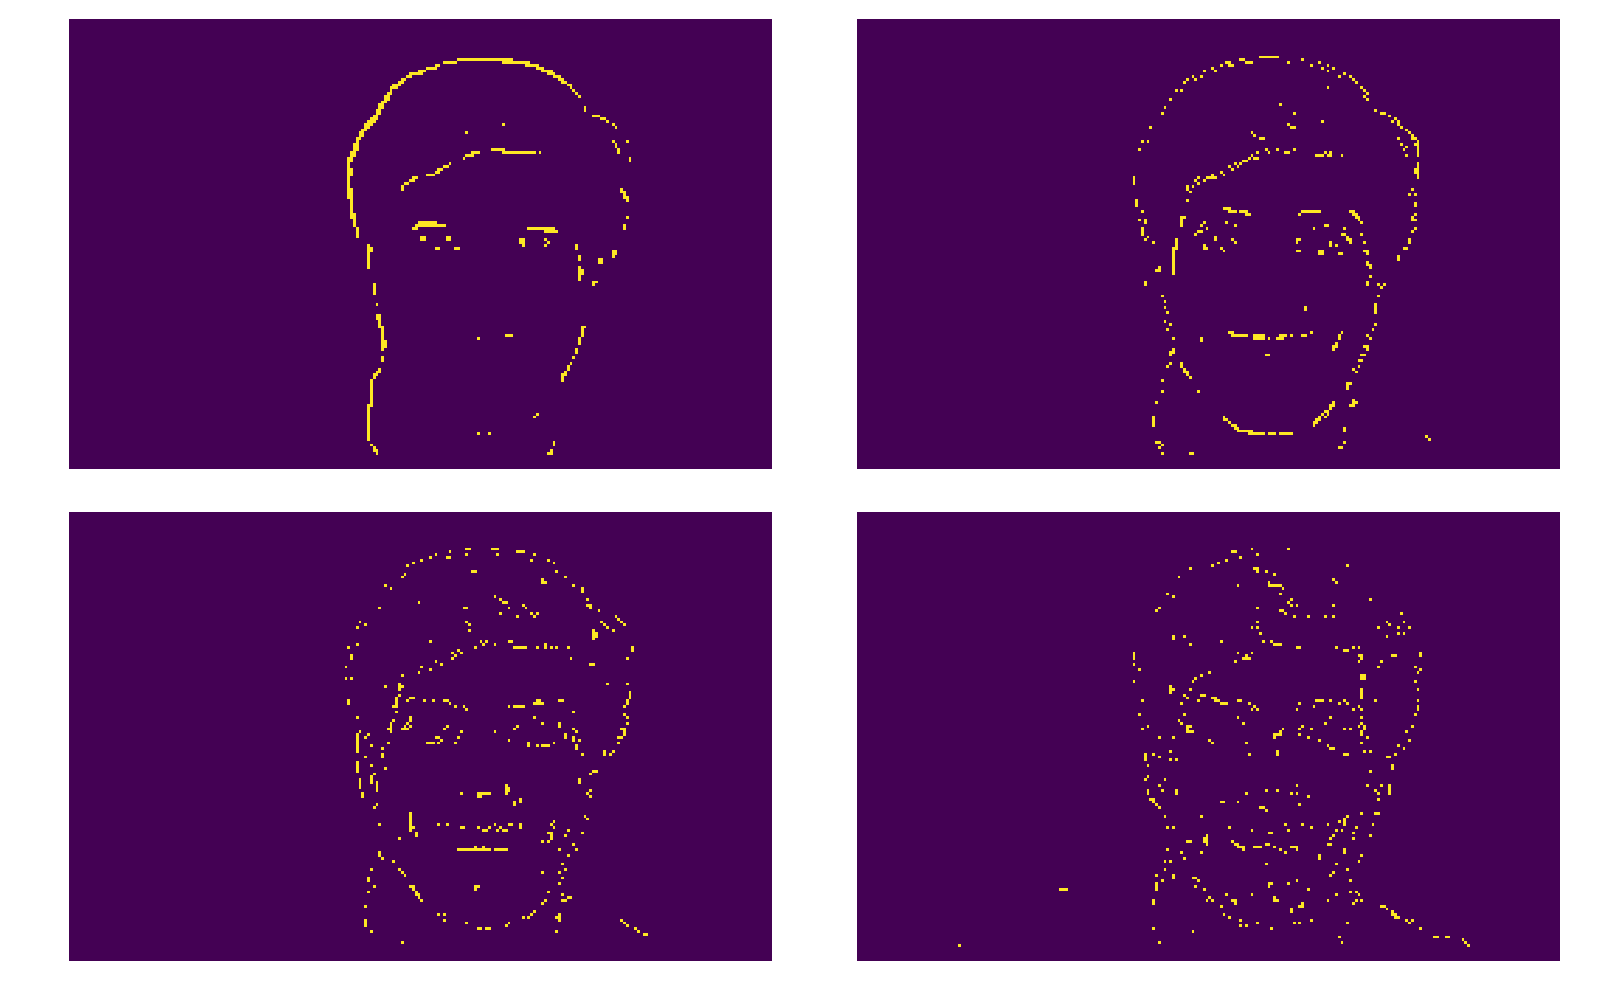
\includegraphics[width=\textwidth]{images/face_dog_out}
		\end{minipage}
	\end{figure}
	\column{.5\textwidth}
	\begin{figure}[!h]
		\centering
		\caption{DoG temporal coding (motorbike)}
		\begin{minipage}[b]{\textwidth}
			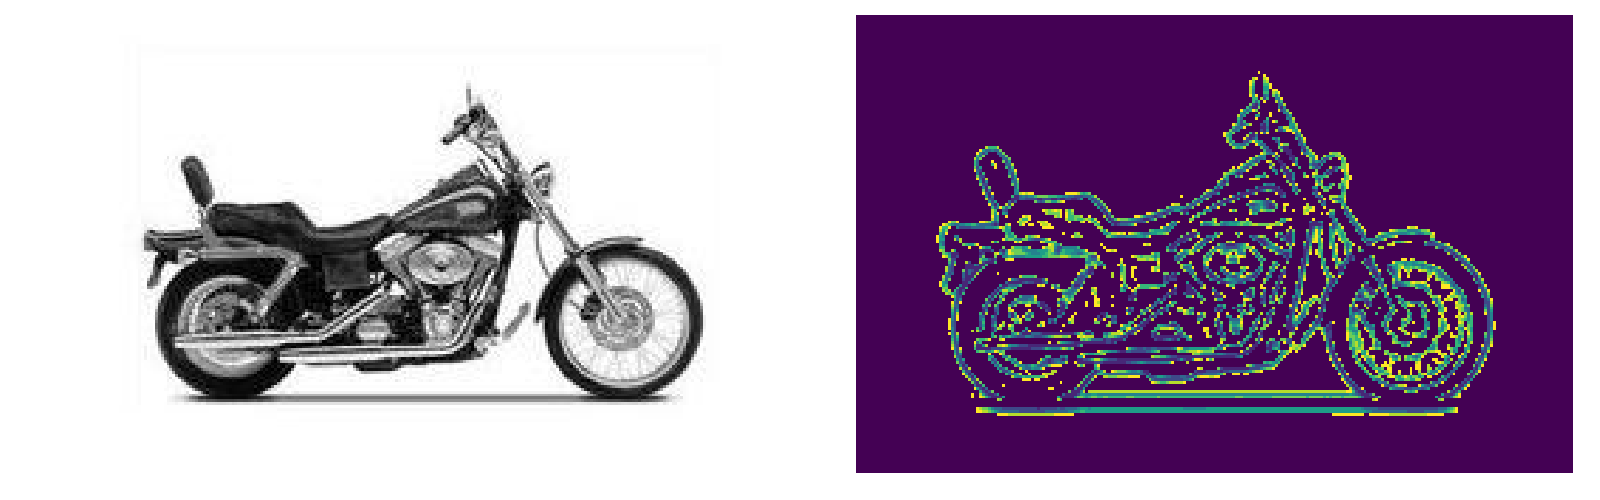
\includegraphics[width=\textwidth]{images/motor_temp}
		\end{minipage}
		\\
		\begin{minipage}[b]{\textwidth}
			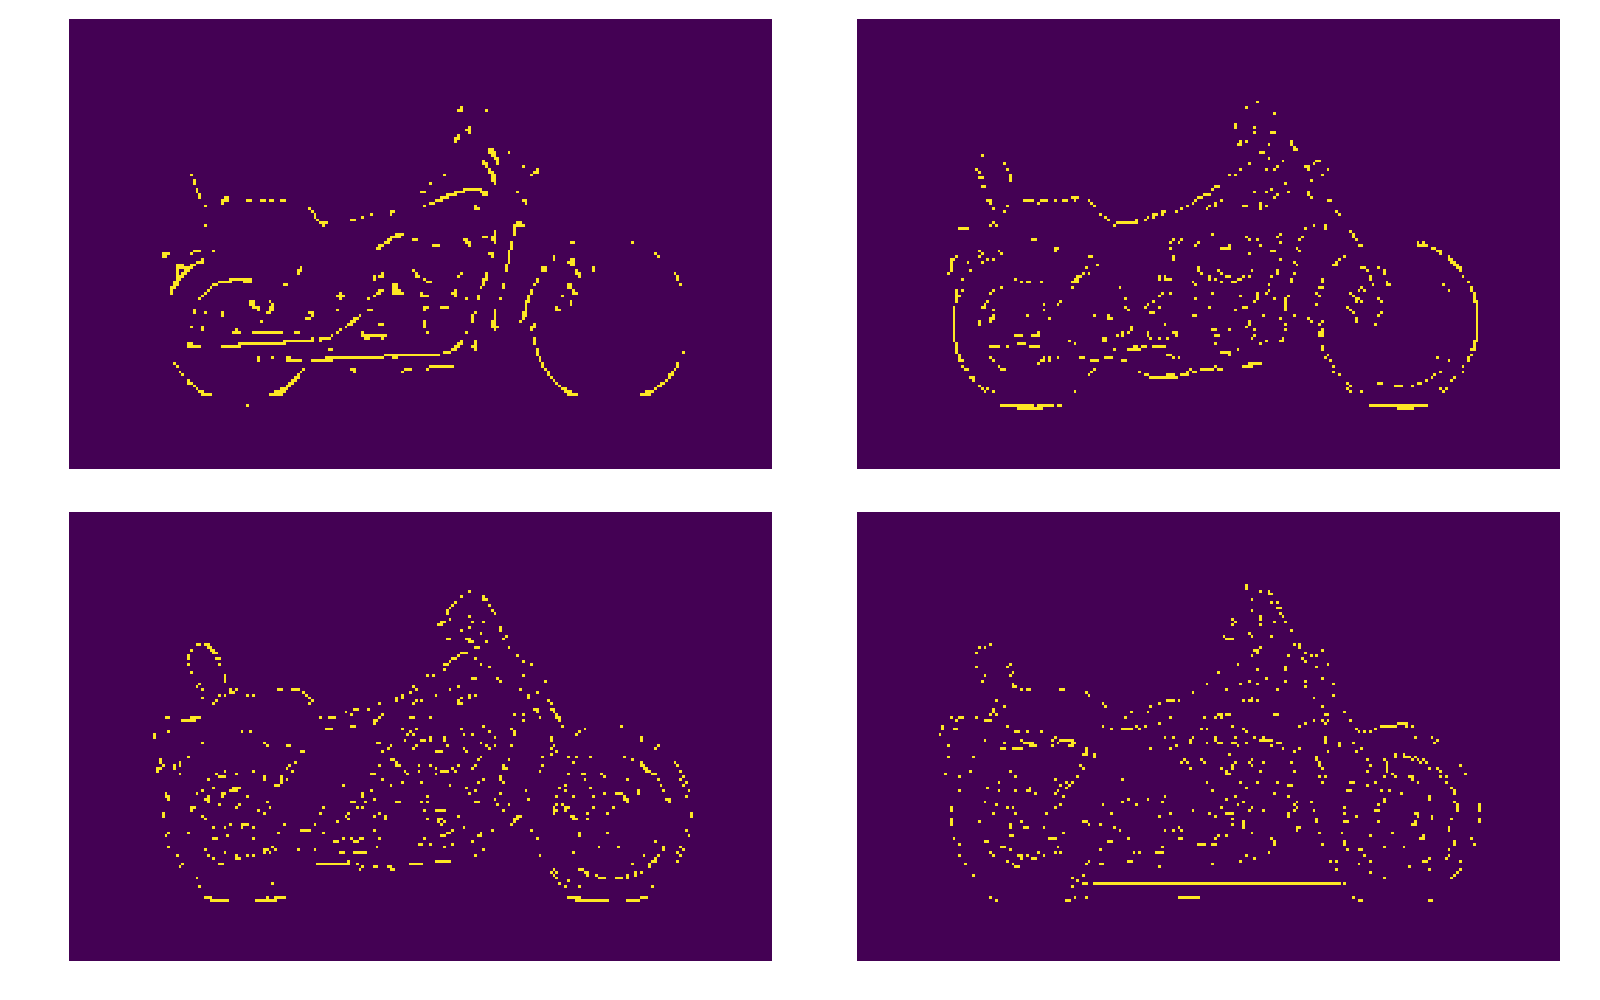
\includegraphics[width=\textwidth]{images/motor_dog_out}
		\end{minipage}
	\end{figure}
\end{columns}
\end{frame}


\begin{frame}{Convolutional layers}

Several neuronal maps detect visual features at different locations.

\begin{itemize}
	\item Same synaptic weights assigned to the	same neuronal maps
	
	\item Neurons generate spikes $ S(t) $ according to the output of the pre-synaptic neurons and when their potential $ V(t) $ exceeds a certain threshold
\end{itemize}

\begin{equation*}
V_{i}(t) = V_{i}(t-1) + \sum_{j}W_{j,i}S_{j}(t-1)
\end{equation*}
\begin{itemize}
	\item After it fires, the neuron can not fire again and it also inhibits other neurons in its same location
\end{itemize}

\end{frame}

\begin{frame}{Convolutional layers}

\begin{figure}[!h]
	\centering
	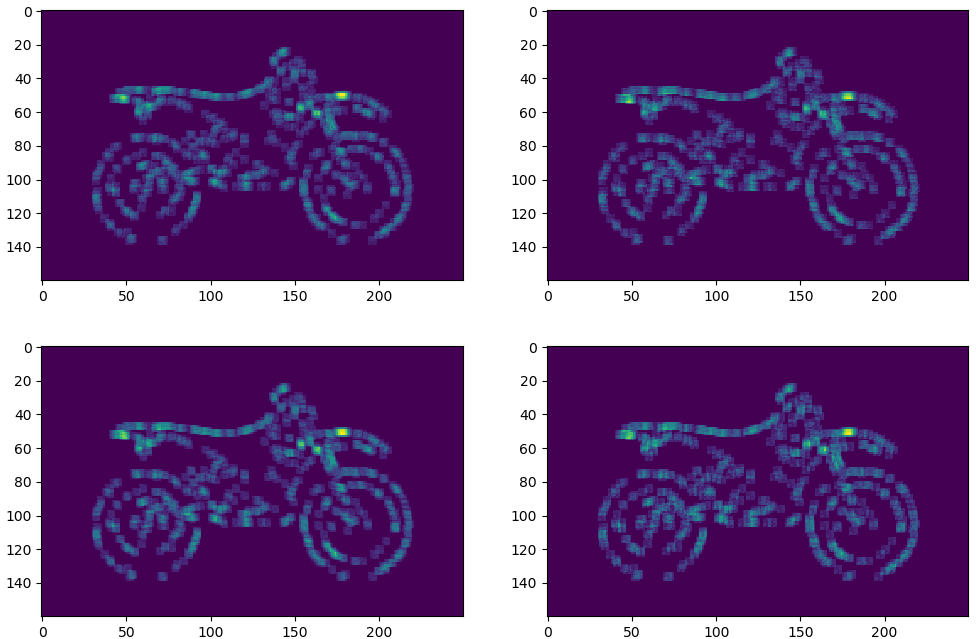
\includegraphics[width=0.9\textwidth]{images/conv_output_slice3_cut}
	\caption{Output of the first convolutional layer}
\end{figure}

\end{frame}

\begin{frame}{Convolutional layers}

\begin{figure}[h]
	\centering
	\caption{Spiking neurons before (top) and after (bottom) inhibition}
	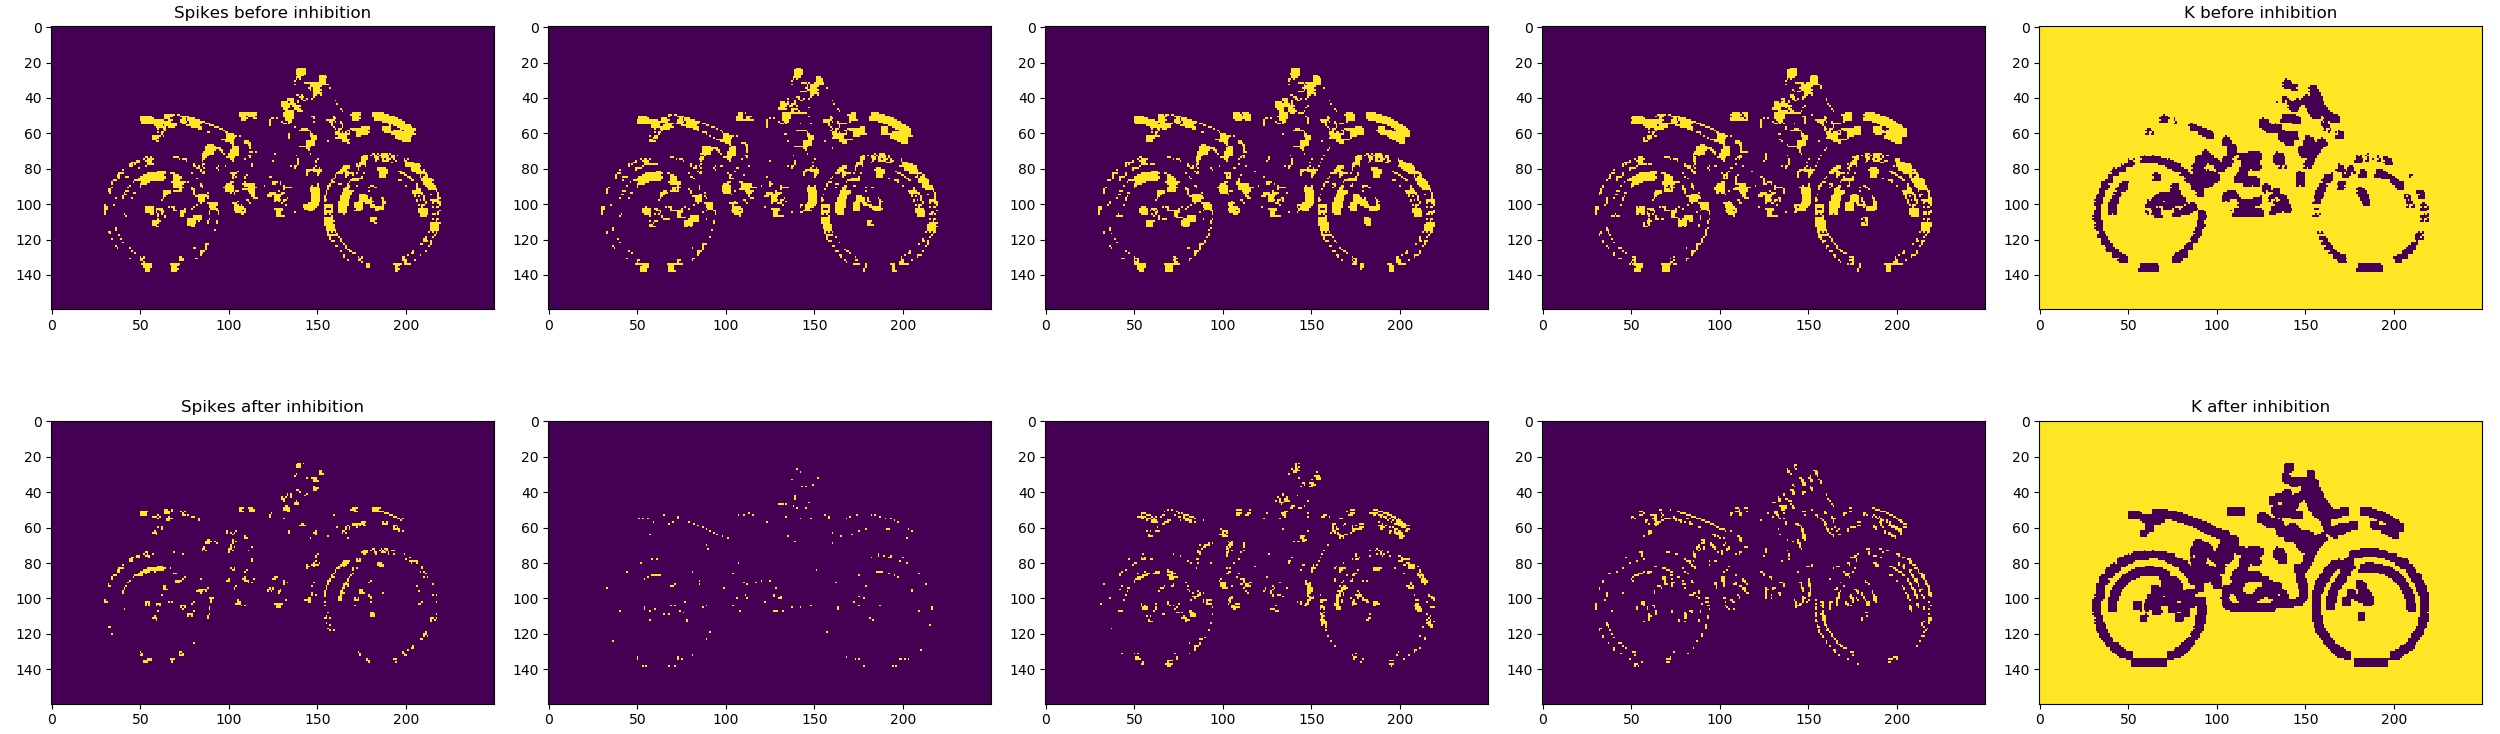
\includegraphics[width=\textwidth]{images/S_K_values_slice2_cut}
\end{figure}
\begin{figure}[h]
	\centering
	\caption{Inhibition matrix for the first three outputs of the DoG filter}
	\begin{minipage}[b]{0.3\textwidth}
		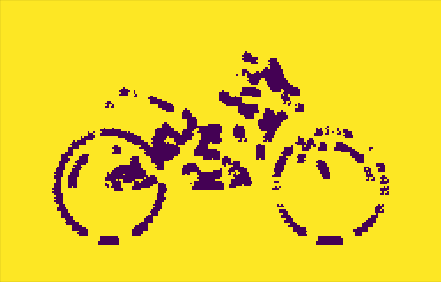
\includegraphics[width=\textwidth]{images/K_1}
	\end{minipage}
	\hfill
	\begin{minipage}[b]{0.3\textwidth}
		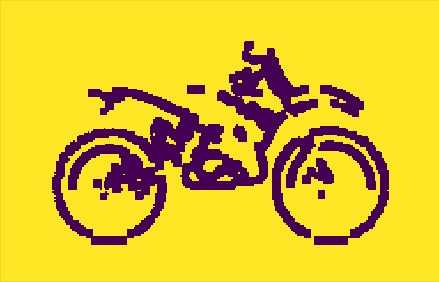
\includegraphics[width=\textwidth]{images/K_2}
	\end{minipage}
	\hfill
	\begin{minipage}[b]{0.3\textwidth}
		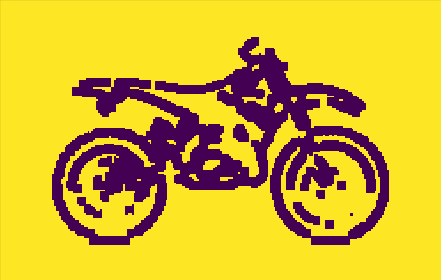
\includegraphics[width=\textwidth]{images/K_3}
	\end{minipage}
\end{figure}

\end{frame}


\begin{frame}{Pooling layers}

Neurons perform a max pooling operation over a window in the corresponding neuronal map of the previous layer.

\begin{itemize}
	\item No learning occurs
	
	\item As before, each neuron can emit only one spike.
	
	\item Visual information
	is compressed
\end{itemize}

\end{frame}

\begin{frame}{Pooling layers}

\begin{figure}[h]
	\centering
	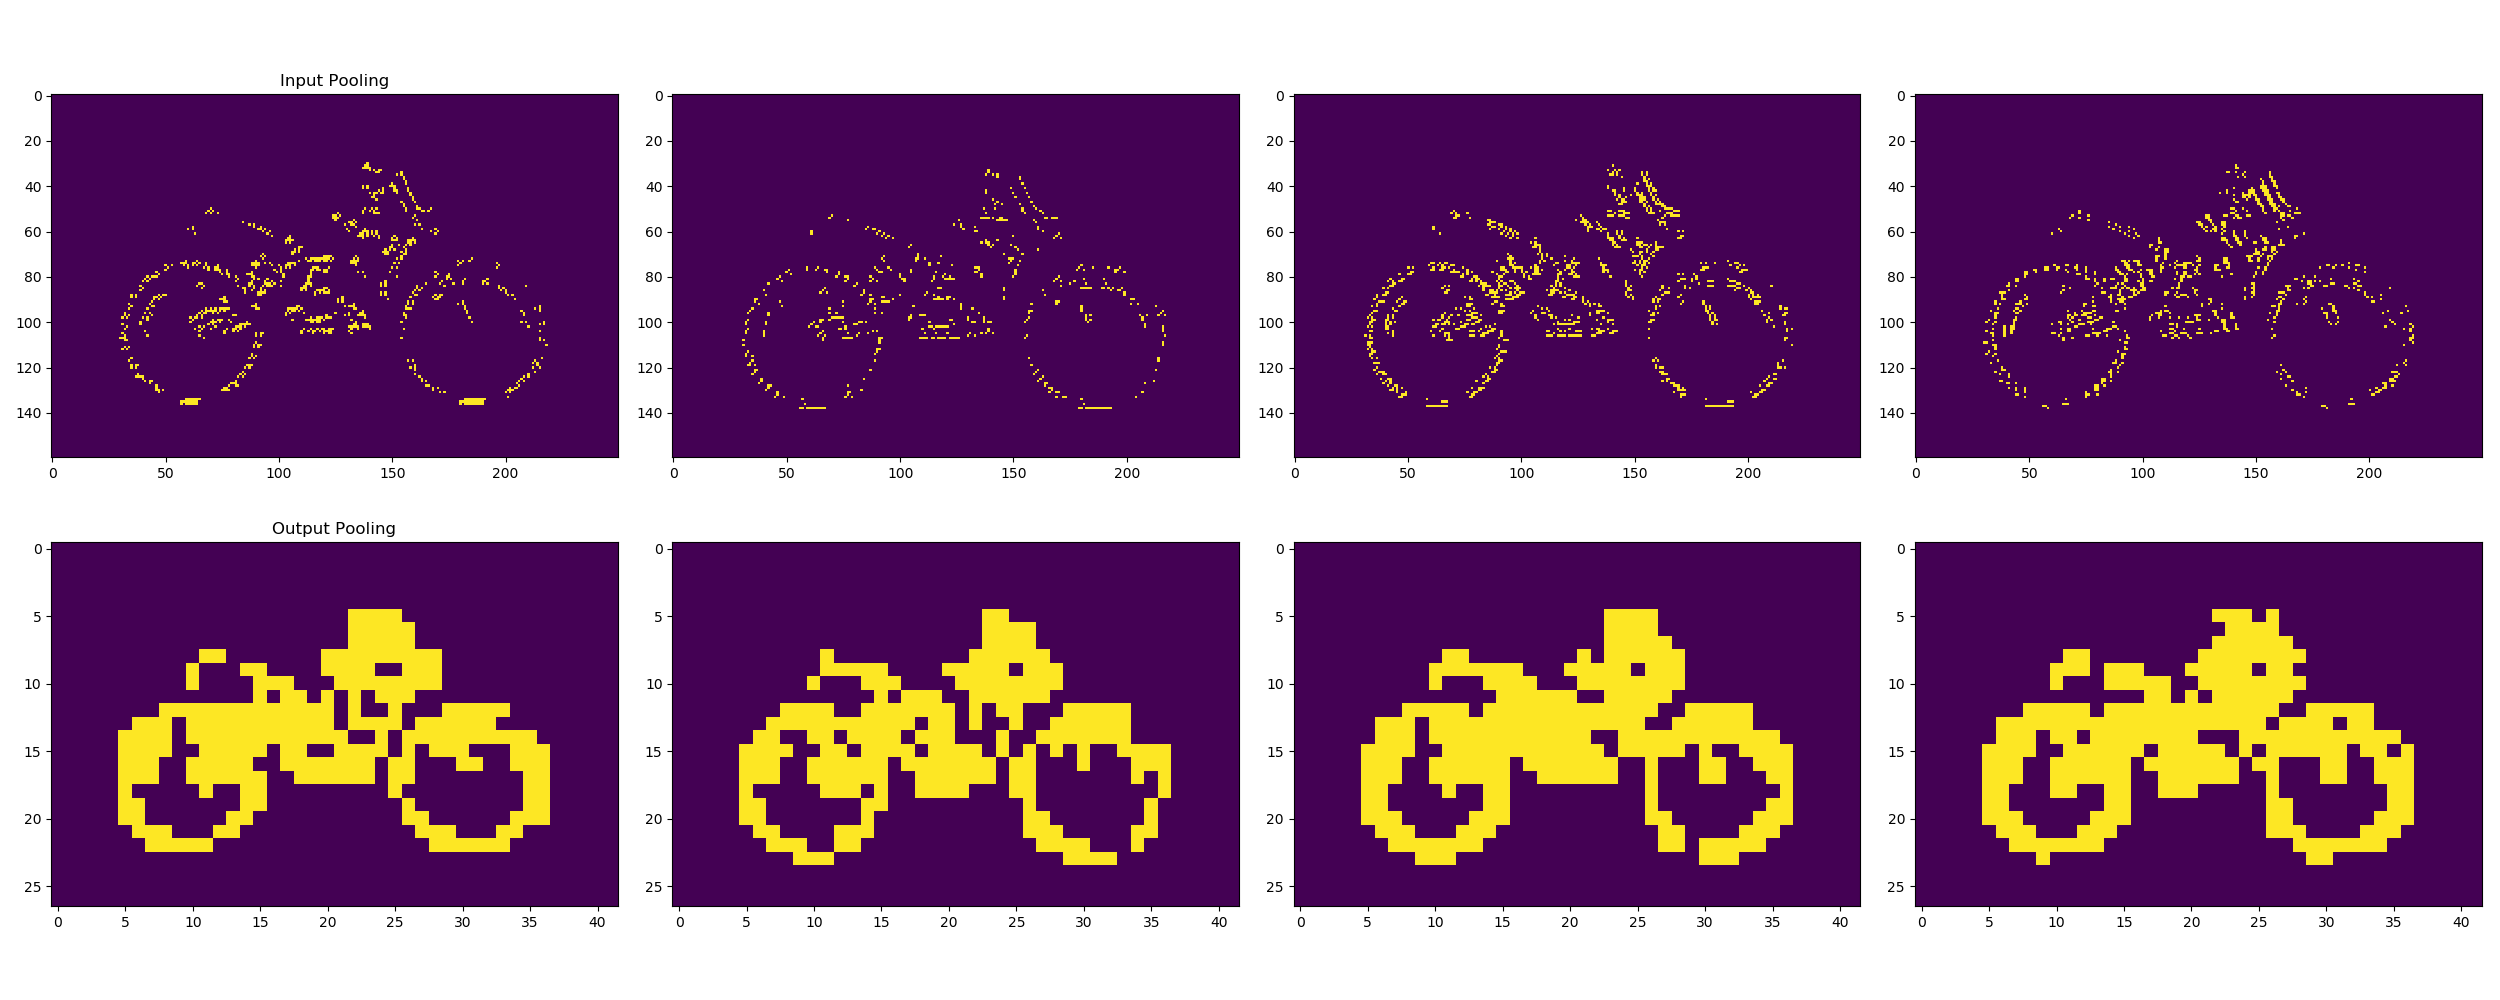
\includegraphics[width=\textwidth]{images/pool_slice1}
	\caption{Input (top) and output (bottom) of the first pooling layer.}
\end{figure}

\end{frame}

\begin{frame}{2nd convolutional layer}

\begin{figure}[h]
	\centering
	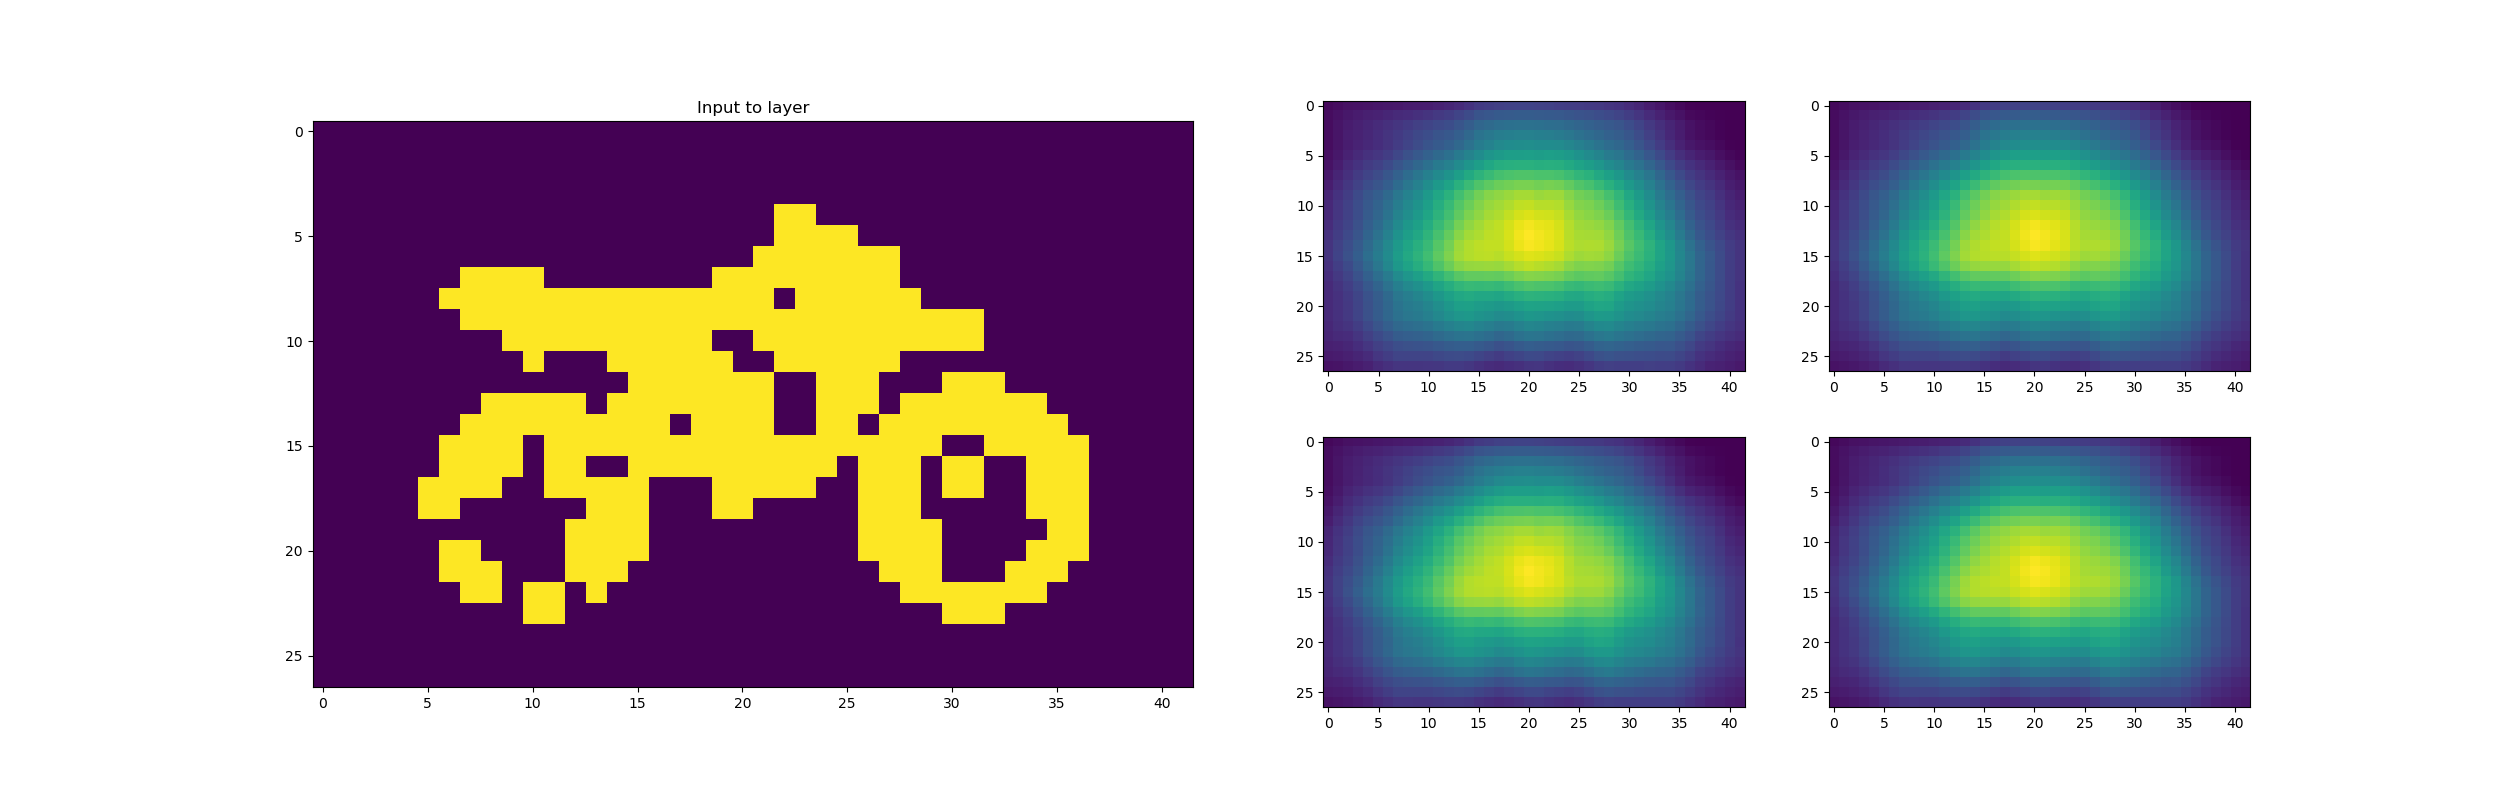
\includegraphics[width=\textwidth]{images/Figure_10}
	\caption{Output of the first pooling layer (left) and of the second convolutional layer (four images)}
\end{figure}

The image is not recognizable any more after the second convolution.

\end{frame}

\begin{frame}{STDP-based learning}

Spike-timing-dependent plasticity (STDP) is a biological process used by brain to modify its own synapses.\\
\bigskip
Here, it allows to strengthen (weaken) synapses if they contribute (or not) to the firing of a post-synaptic neuron.
\begin{figure}[h]
	\centering
	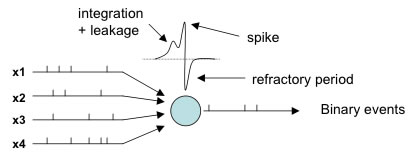
\includegraphics[width=0.8\textwidth]{images/spikes}
\end{figure}

\end{frame}

\begin{frame}{STDP-based learning}

Learning occurs only in convolutional layers, so that neurons compete to fire earlier than others and use STDP to learn input patterns.\\
\bigskip
STDP is represented by:
\begin{equation*}
\Delta w_{ij} = \begin{cases}
a^{+}w_{ij}(1-w_{ij}), & \textit{if }\; t_{j}-t_{i} \leq 0,\\
a^{-}w_{ij}(1-w_{ij}), & \textit{if }\; t_{j}-t_{i} > 0,
\end{cases}
\end{equation*}

where $ \Delta w_{ij} $ is the synaptic weight modification and $ a^{+} $ and $ a^{-} $ are the learning rate parameters. 

\end{frame}

\begin{frame}{STDP-based learning}

Weights are randomly initiated with $ \mu = 0.8 $ and $ \sigma = 0.05 $.\\
\bigskip
The learning convergence of the \textit{l-th} convolutional layer is represented by:

\begin{equation*}
C_{l} = \sum_{f}\sum_{i}w_{f,i}(1-w_{f,i})/n_{w}
\end{equation*}

where $ n_{w} $ is the total number of synaptic weights in that layer and $ w_{f,i} $ is the \textit{i-th} synaptic weight of the \textit{f-th} feature.

\end{frame}

\begin{frame}{STDP-based learning}

\begin{figure}[!h]
	\centering
	\begin{minipage}[b]{\textwidth}
		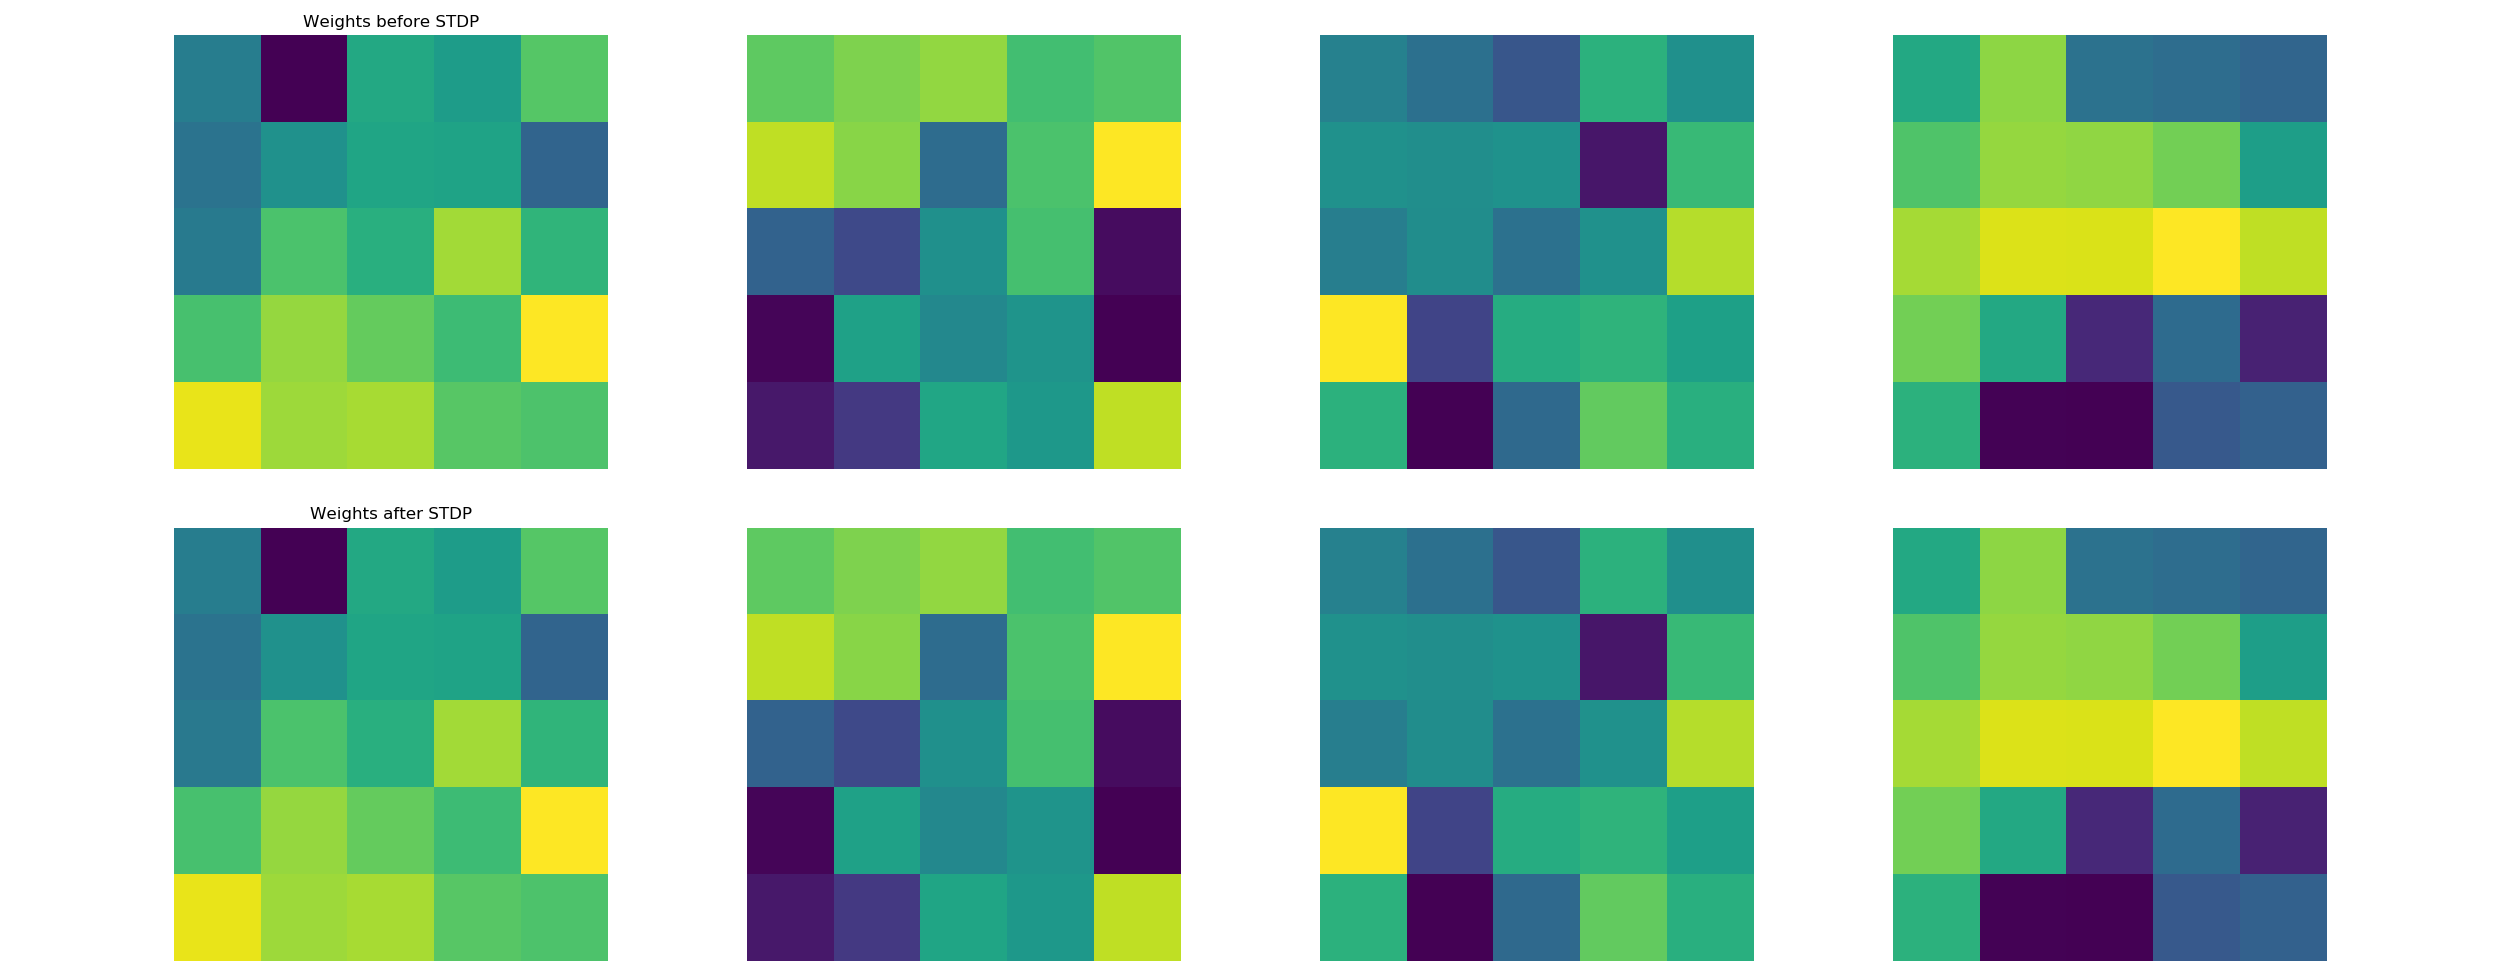
\includegraphics[width=\textwidth]{images/Figure_15}
	\end{minipage}
	\\[0.5em] \begin{minipage}[b]{\textwidth}
		
\includegraphics[width=\textwidth]{images/3Figure_15}
	\end{minipage}
	\hfill
	\caption{Weights randomly initialised (top) and updated after one (middle) and three images processed (bottom).}
\end{figure}

\end{frame}

\begin{frame}{Classification}

The output of the global max pooling layer is used to build a dataset of labelled
features which are split in a training and testing set for the classifier.\\
\bigskip
Features are the greatest potentials reached by the neuronal maps in the third convolutional layer.\\
\bigskip
The resulting dataset is standardised and used to feed a linear SVM.

\end{frame}

\section{Conclusion}

\begin{frame}{Summary}

\begin{itemize}
	\item New \textit{spiking} neuron models used to handle a bio-inspired neural network.\\
	\bigskip
	\item Spatio-temporal information acquired in a better way and good results obtained with few input data\\
	\bigskip
	\item 88\% of accuracy with some existing functions\\
	62\% - 75\% (depending on the parameters and the classifier) with every function implemented from scratch
\end{itemize}

\end{frame}

\begin{frame}{Possible improvements}

\begin{itemize}
	\item Modify the STDP, in order to apply penalty on more neurons not involved in the spiking process\\
	\bigskip
	\item Extend the encoding time of the DoG filter to have a better differentiation between useful and useless information  (side-effect of computational effort)

\end{itemize}

\end{frame}

\begin{frame}{References}

\begin{thebibliography}{3}	
  \bibitem{STPD}   S. R. Kheradpisheh, M. Ganjtabesh, S. J. Thorpe, and
  T. Masquelier, "Stdp-based spiking deep convolutional neural
  networks for object recognition," Neural Networks, vol. 99,
  pp. 56–67, 2017.
  \\[1.2em]
  \bibitem{Next-gen}
  Spiking Neural Networks, the Next Generation of Machine Learning, https://towardsdatascience.com/spiking-neural-networks-the-next-generation-of-machine-learning-84e167f4eb2b
  \\[1.2em]
  \bibitem{GitHub}
  Spiking-Neural-Network, https://github.com/Shikhargupta/Spiking-Neural-Network
\end{thebibliography}

\end{frame}

\end{document}
